% chapitre dédié au nuage
\chapter{Utiliser le nuage}
%\addcontentsline{toc}{chapter}{Utiliser le nuage}

Le ``Nuage'' est le nom qui a été donné à l'espace de stockage en ligne, actuellement d'une taille maximale de 100~Go\footnote{%
100~Go = 100 milliards de caractères simples.
} 
offrant en outre la présence d'une suite bureautique en ligne --libreoffice en ligne ou lool-- et d'éditeurs avancés de texte enrichi.

Le nuage est accessible de deux façons différentes pour l'instant --j'espère que la troisième fonctionnera aussi bientôt--~: \emph{via} l'interface web (firefox, chrome, edge, autres ...) ou \emph{via} le client \emph{nextcloud}.

Même si les avis divergent entre \emph{bloggers\/} au sein du vaste monde d'internet, il y a un adage que beaucoup partagent~: \og~\emph{There is no cloud : it's just someone else's computer.\/}\footnote{Il n'y a pas de Nuage : c'est seulement l'ordinateur de quelqu'un d'autre.}~\fg{}. 
En effet malgré que peut apporter un \emph{data center\/} ou un \emph{cluster} de telles structures en terme de répartition, si la société qui gère tout ce stockage distant décide de fermer le service, vous n'y aurez plus accès.

\section{L'interface Web}
%\addcontentsline{toc}{section}{L'interface web}

L'interface web est celle qui sera sans doute la plus utilisée car dès que l'on est en établissement scolaire, peu importe les blocages ou les applications, la certitude de trouver un navigateur dans chaque ordinateur est quasi absolue.
\begin{figure}
	\centering
	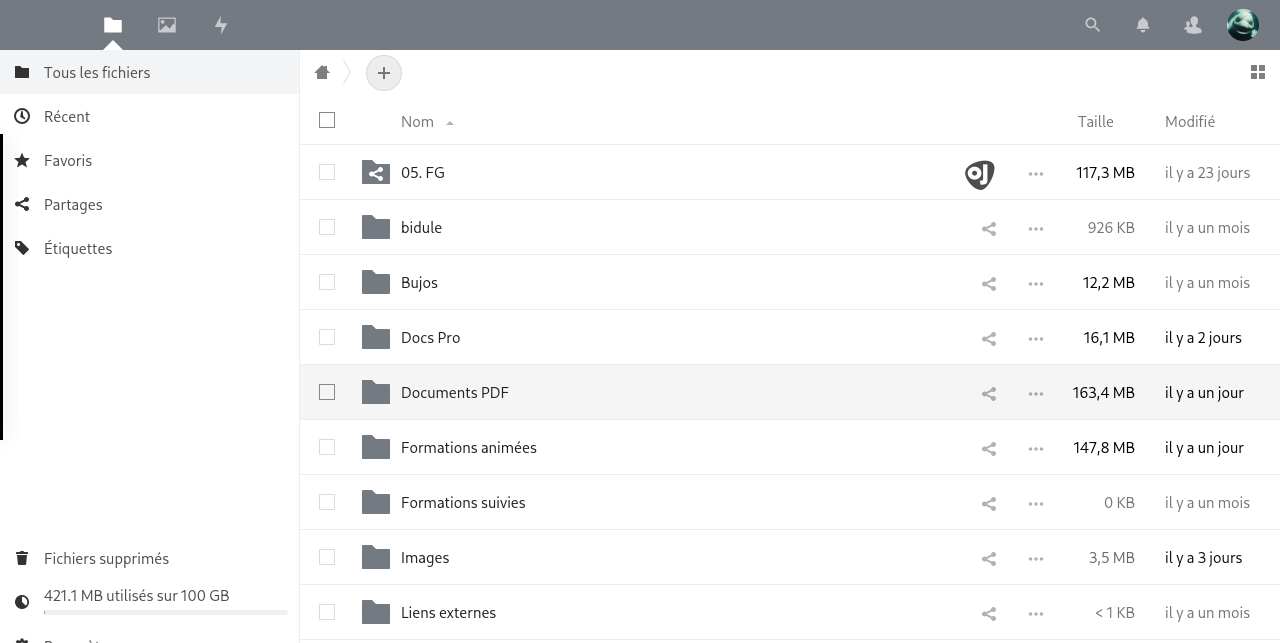
\includegraphics[width=\linewidth]{./Captures/nuage.accueil.png}
	\caption{Le nuage en mode détaillé}
\end{figure}
L'interface est visible en mode mosaïque également.
\begin{figure}
	\centering
	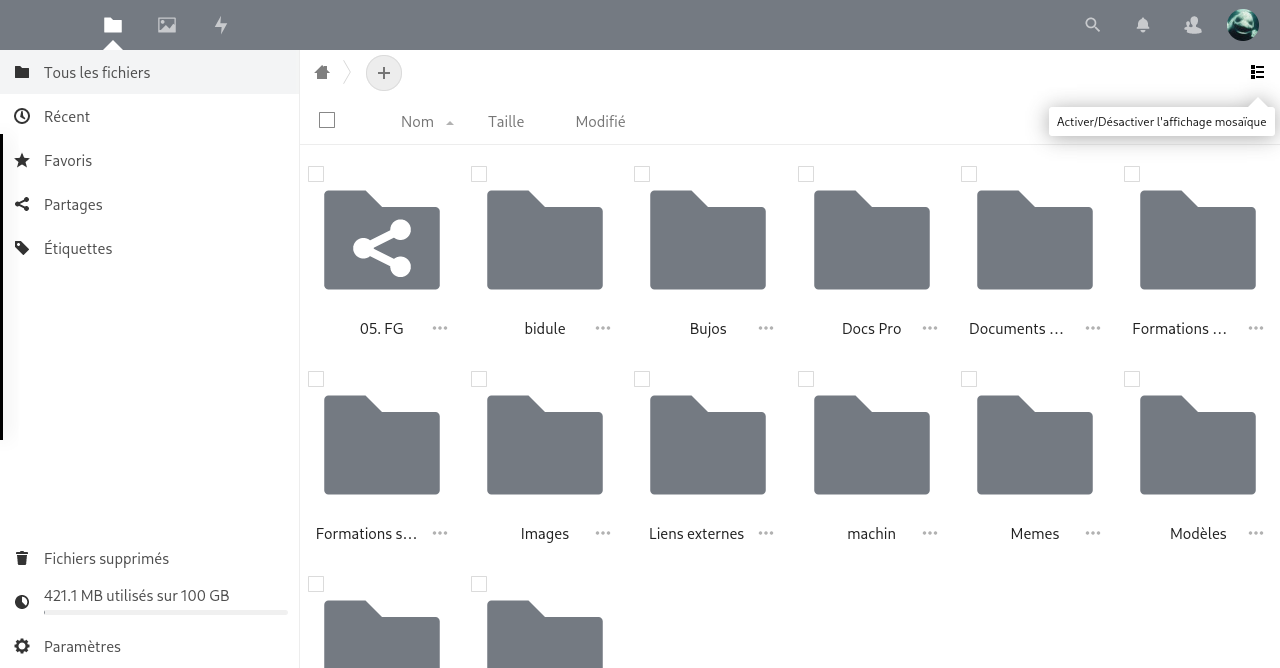
\includegraphics[width=\linewidth]{./Captures/nuage.accueil.mozaique.png}
	\caption{Le nuage en mode mosaïque.}
\end{figure}
L'intérêt de cette interface est de pouvoir y déposer ou récupérer un ou plusieurs fichiers, ou bien un ou plusieurs dossiers. 
L'autre intérêt est que le site étant en ``education.fr'' il ne sera donc pas filtré par les systèmes de pare-feu académiques et évitera l'emploi de clés USB qui se promènent entre le domicile et l'établissement où les niveau de sécurité sont très différents.



\section{Le client NextCloud}
%\addcontentsline{toc}{section}{Le client nextcloud}
Le nuage de \emph{apps} est basé sur le travail d'un groupe important de développeurs et de développeuses qui ont fondé le site et le serveur ``Nextcloud''. 
Ce service en ligne permet outre ce qui est offert par le nuage bien d'autres fonctionnalités. 

\begin{multicols}{2}

\begin{figure}
	\centering
	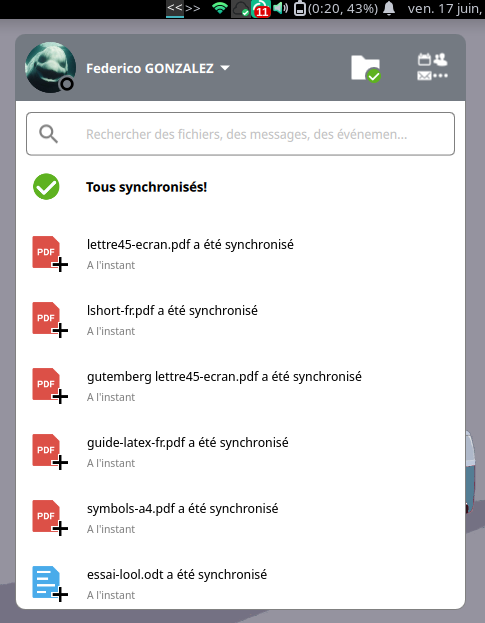
\includegraphics{./Captures/nextcloud-client.fenetre.principale.png}
	\caption{Le client pour PC (MacOS, Windows, ici : Linux}
\end{figure}

\columnbreak

\begin{figure}
	\centering
	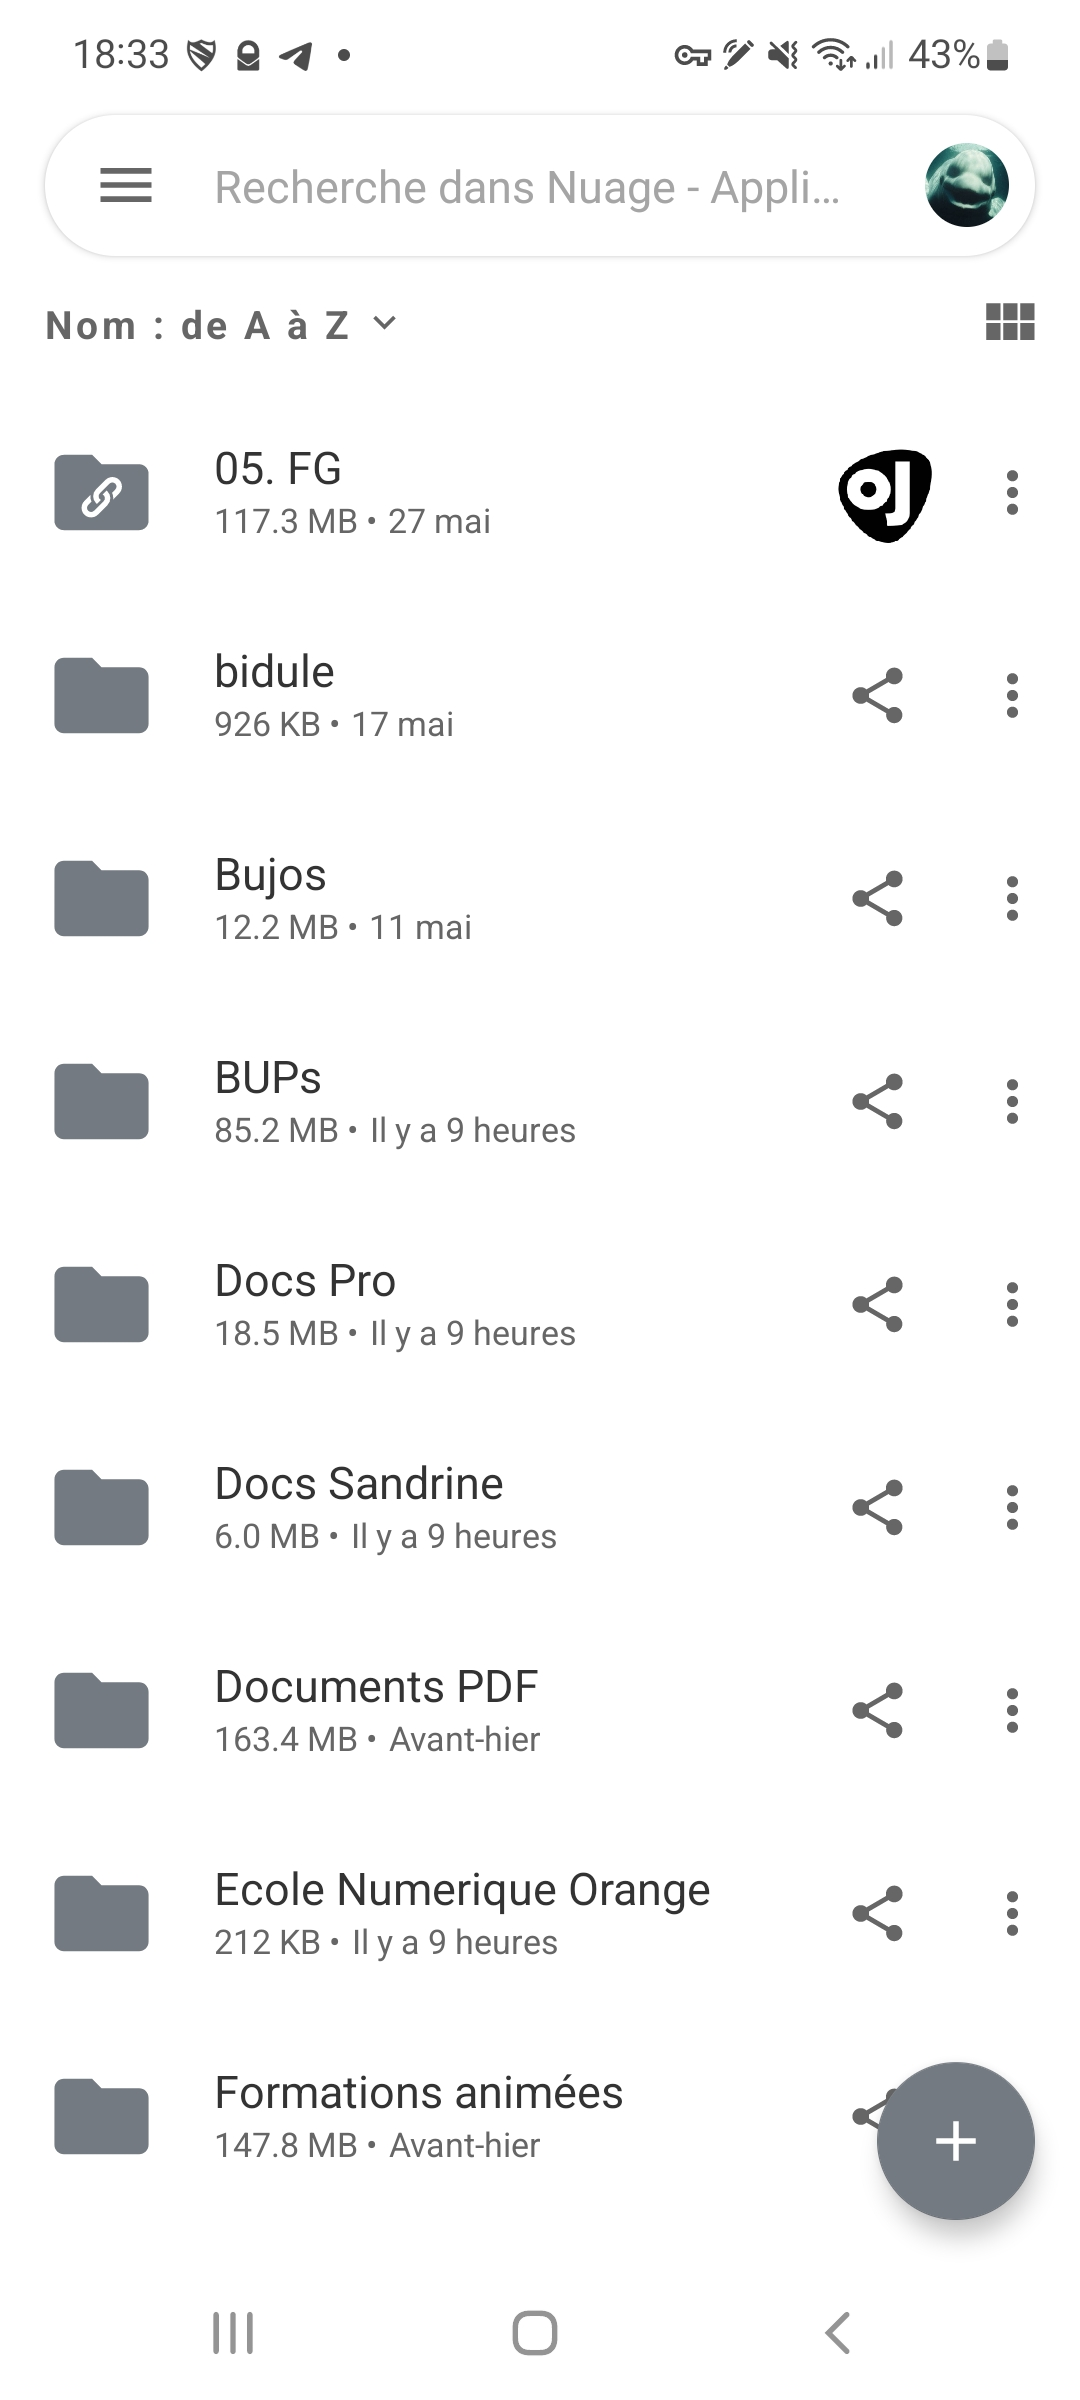
\includegraphics{./Captures/nextcloud-client.smartphone.jpg}
	\caption{Le client Nextcloud pour smartphone, version Android.}
\end{figure}
\end{multicols}
L'application est bien sûr disponible sur votre \emph{store\/}, quant au programme pour ordinateur il suffit d'aller sur le site \url{https://www.nextcloud.com} dans la section téléchargement.

Comment fonctionne le client Nextcloud pour PC~? 
C'est assez facile à comprendre. 
Lors de son installation, le client va demander un dossier, soit par défaut, soit en le spécifiant et en le créant, afin que tout fichier ou tout dossier qui y sera créé, supprimé, modifié, renommé, déplacé ou copié, sera synchronisé également sur le serveur automatiquement.
\begin{figure} \label{fig-dossier-synchro}
	\centering
	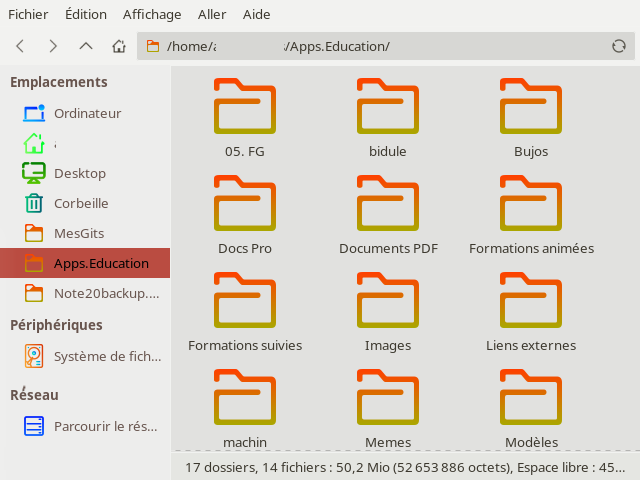
\includegraphics{./Captures/nextcloud-client.dossier.synchronise.png}
	\caption{Le dossier synchronisé sur mon P.C.}
\end{figure}

\paragraph{Notez.} 
Les prochaines sections et sous-sections traiteront de l'outil qui sera le plus souvent utilisé à savoir le transfert et la création d'objets par l'interface web, la gestion de tels échanges par le client nextcloud sera vu dans d'autres sections ultérieurement.

\section{Transfert de données}
%\addcontentsline{toc}{section}{Transfert de données}
Le transfert de fichiers et de dossiers entre périphériques est possible depuis plusieurs sources et selon plusieurs protocoles. 
L'image qui suit montre une synchronisation à double sens en utilisant le logiciel sur P.C. --~flèches en rose~--, ou bien via le navigateur --~flèches en bleu~-- ou encore via l'application d'un smartphone ou d'une tablette --~flèches en rouge.
\begin{figure}
	\centering
	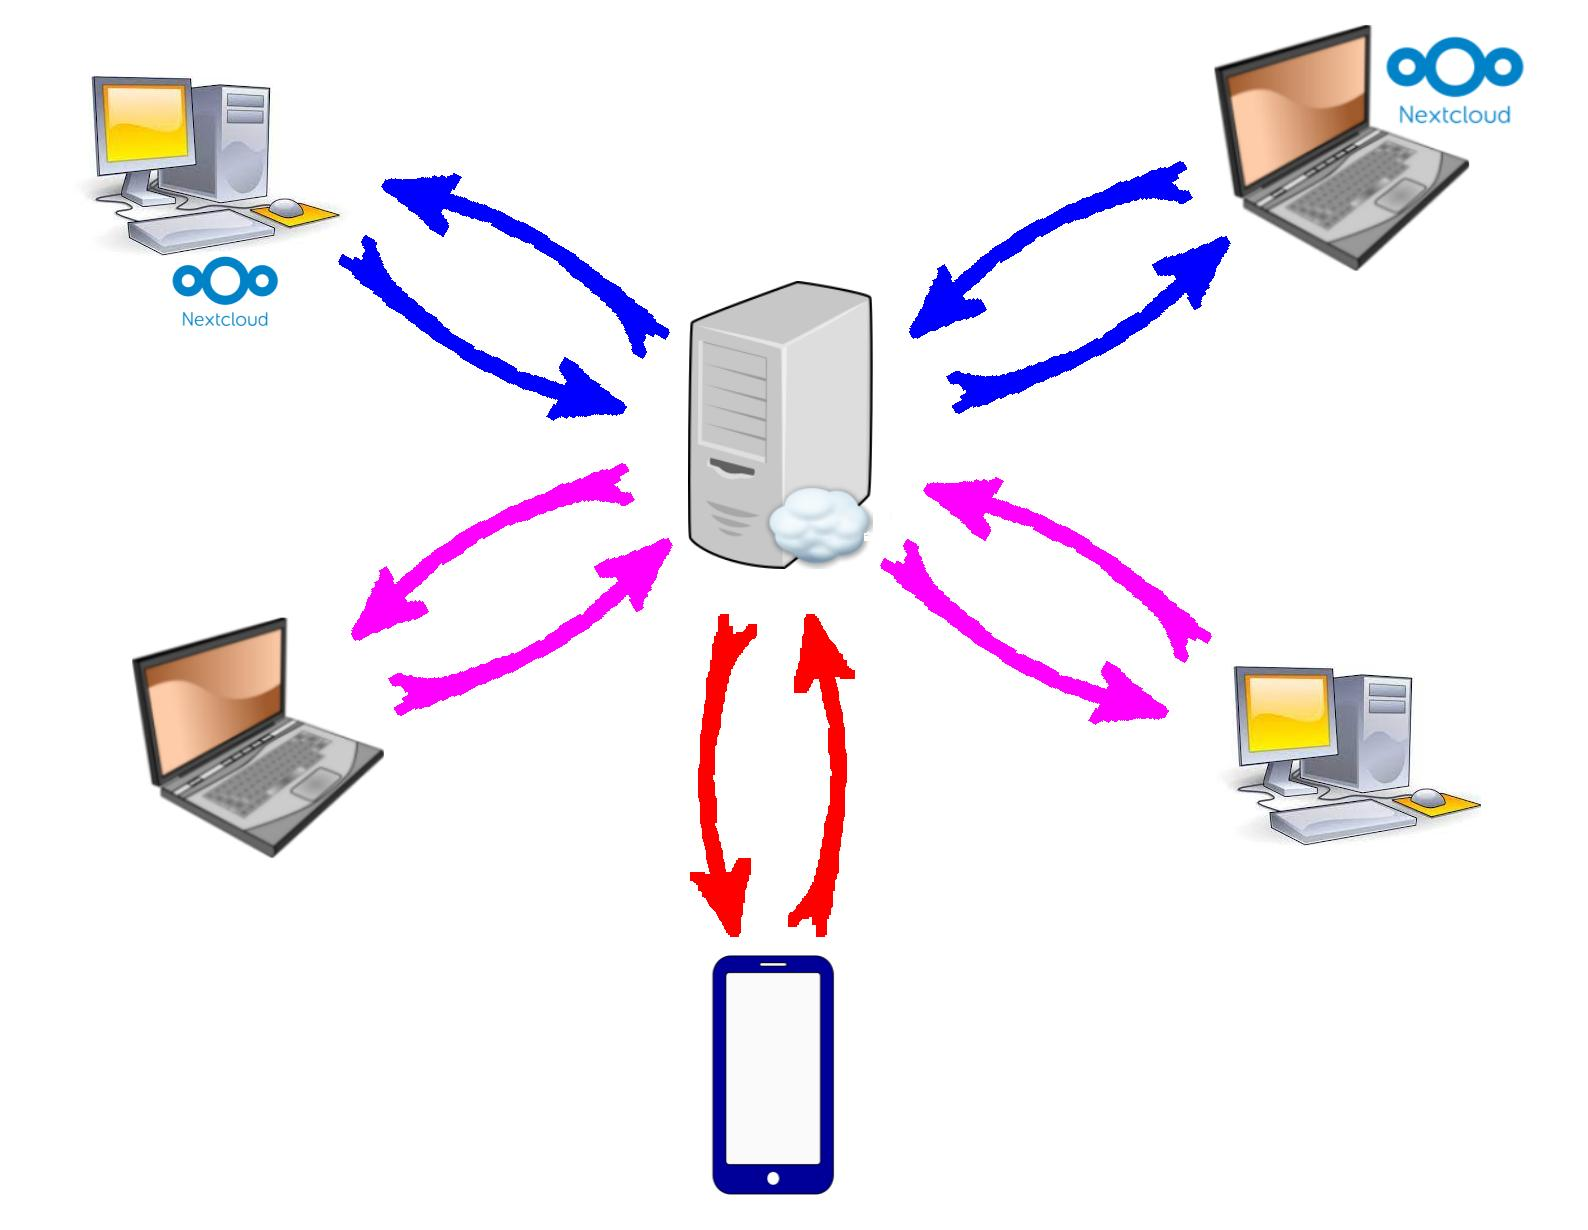
\includegraphics{./Captures/synchro.nextcloud.nuage.jpg}
	\caption{Le nuage est accessible par l'outil Nextcloud, par le navigateur, ou par le client smartphone pour transférer des données dans les deux sens.}
\end{figure}

\paragraph{La synchronisation via le client nextcloud pour ordinateur.} 
Comme le montre la capture d'écran du paragraphe \ref{fig-dossier-synchro}, transférer des fichiers entre l'ordinateur personnel et le nuage revient simplement à copier ou déplacer fichiers ou dossiers vers le dossier synchronisé, en soi on peut supposer que cette compétence est acquise par chaque lecteur.

Aussi dans les sous-sections suivantes ne seront abordés que le transfert de fichier par l'interface web.
De plus j'utiliserai le terme ``monter'' en lieu et place de l'anglicisme \emph{upload} et ``descendre'' parfois au lieu de télécharger.

\subsection{Monter un ou plusieurs fichiers}
%\addcontentsline{toc}{subsection}{Monter un ou plusieurs fichiers}
Tout se passe par l'icône en forme de rond avec une croix à l'intérieur, le {\Large $\oplus$} à gauche de la barre horizontale au dessus de l'espace réservé pour afficher les fichier. L'appui sur l'icône affiche le menu de la capture suivante~:
\begin{figure}
	\centering
	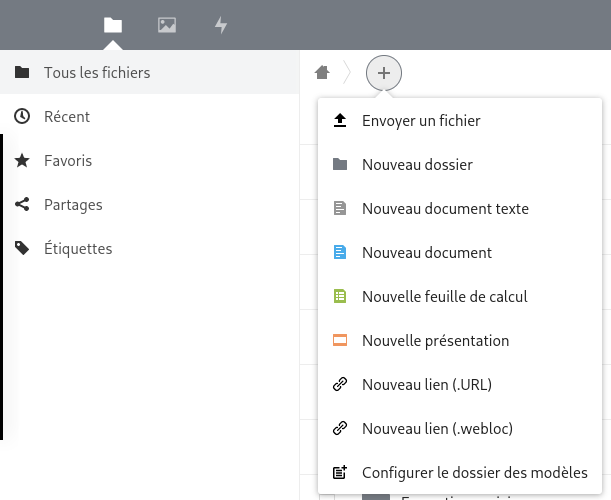
\includegraphics[width=0.5000\linewidth]{./Captures/nuage.menu.plus.png}
	\caption{Le menu ``plus''}
\end{figure}
En cliquant sur la ligne \og~Envoyer un fichier~\fg{} une fenêtre de l'explorateur local va s'ouvrir permettant de sélectionner un ou plusieurs fichiers qui seront envoyés dans le dossier affiché à l'écran.

\subsection{Créer un dossier}
%\addcontentsline{toc}{subsection}{Créer un dossier}
En cliquant sur la deuxième ligne du menu déroulant, c'est la création d'un dossier dans le dossier courant, attention il faut penser à clique sur la flèche au bout de la ligne pour valider le nom et créer le dossier.
\begin{figure}
	\centering
	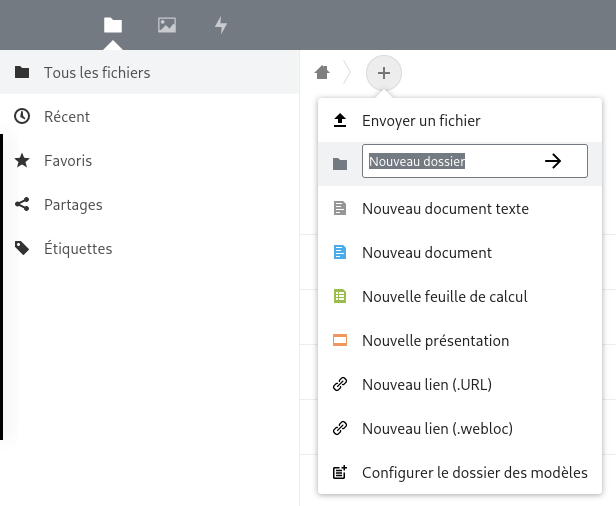
\includegraphics[width=0.5000\linewidth]{./Captures/nuage.menu.plus.creer.dossier.png}
	\caption{}
\end{figure}

Afin de valider la création d'un dossier, il suffit de saisir son nom et de valider par la touche entrée ou bien en cliquant sur la flèche en bout de ligne $\rightarrow$ et le dossier sera créé dans le dossier courant.

\subsection{Descendre un dossier ou plusieurs fichiers}
%\addcontentsline{toc}{subsection}{Descendre un dossier ou plusieurs fichiers}
L'un des avantages du nuage intégré à Apps.Education est la possibilité d'ouvrir, certes, mais aussi de télécharger ensuite un ou plusieurs fichiers, ou bien un ou plusieurs dossiers.

\begin{figure}
	\centering
	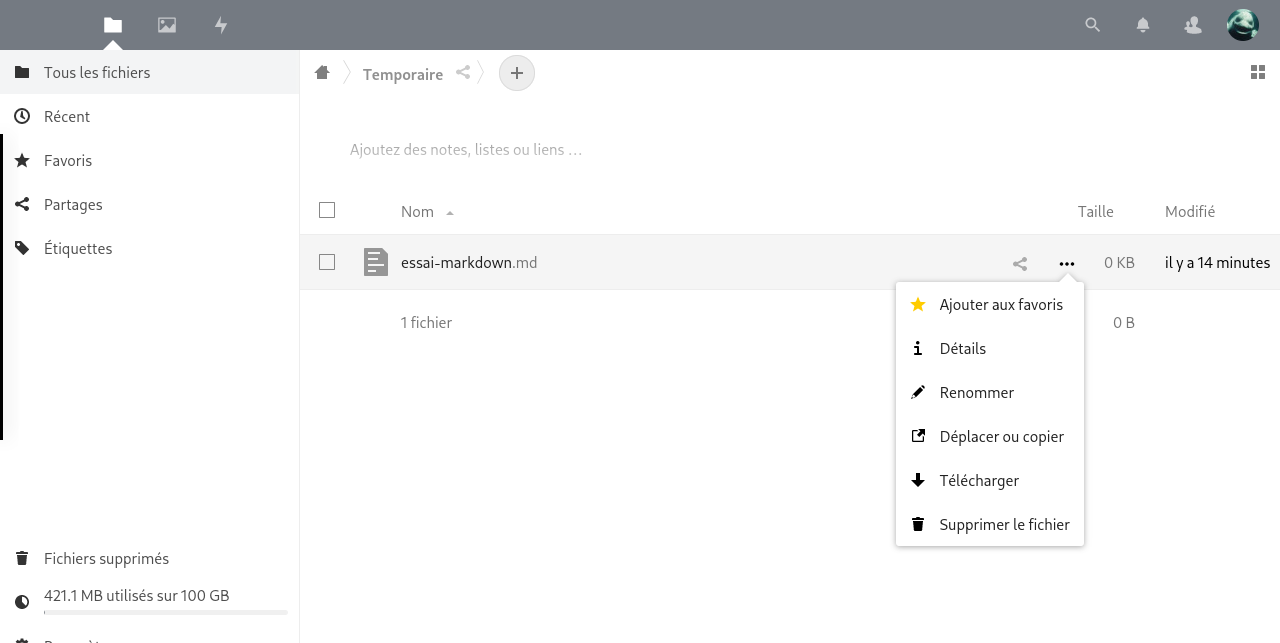
\includegraphics{./Captures/nuage.accueil.menu.contextuel.png}
	\caption{}
\end{figure}
Lorsqu'on appuie sur les \ldots un menu contextuel montre les différents choix proposés pour cet objet --~ici un fichier un texte balisé en langage \texttt{Markdown}. 

\subsection{Ce qui est spécifique au programme Nextcloud}
%\addcontentsline{toc}{subsection}{Ce qu'il n'est pas possible de faire} 
Par défaut, l'interface web du nuage ne permet pas d'envoyer directement un dossier, son contenu et toute la hiérarchie fille qui en découle, mais, cela reste possible par l'utilisation du client Nextcloud vu précédemment. 

Ouvrez deux fenêtres, l'une pointant le dossier synchronisé par le client Nextcloud, l'autre montrant la source des données à transférer, et, comme vous le feriez d'un dossier vers un dispositif externe, copiez ou déplacez les objets choisis (mélangeant tout ce que vous voulez de dossiers et de fichiers), quelques instants plus tard la synchronisation s'effectuera et créera dans le nuage les dossiers, les sous-dossiers et y placeront tous les fichiers quelque soit leur position dans l'arborescence.

Parmi les choix proposés, on peut renommer le fichier, le copier ou le déplacer --~c'est la même fenêtre mais pas le même bouton sur lequel cliquer~-- ou encore télécharger la ressource.

La règle est simple, si la ressource est un fichier simple, le fichier est téléchargé tel quel si par contre cela correspond à la sélection de plusieurs objets ou au moins d'un dossier, alors le nuage va compresser le tout dans une ressource unique, un fichier \emph{.zip} et c'est cet élément qui sera téléchargé.

\paragraph{Notez aussi.} 
On peut sélectionner un ou plusieurs objets en cliquant sur la case $\square$ en début de ligne, faisant apparaître en haut, à droite de \og~Nom~$\triangledown$~\fg{} comme le montre l'image qui suit.
\begin{figure}
	\centering
	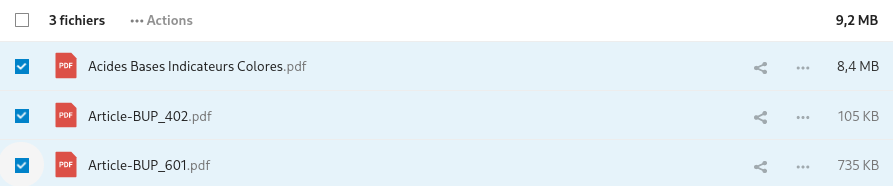
\includegraphics{./Captures/nuage.selection.plusieurs.objets.png}
	\caption{Sélection de plusieurs objets}
\end{figure}
on peut aussi sélection tous les objets du répertoire en cliquant sur le $\square$ tout en haut.
\begin{figure}
	\centering
	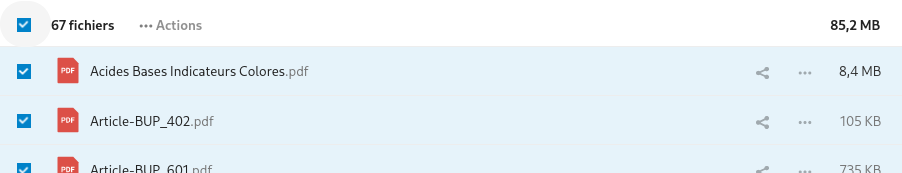
\includegraphics{./Captures/nuage.selection.tous.objets.png}
	\caption{Sélection complète}
\end{figure}

\section{Partager une ressource}
%\addcontentsline{toc}{section}{Partager une ressource} 
Tout document posé dans le nuage, que ce soit un simple fichier ou bien un dossier à un ou plusieurs sous-niveaux est une ressource pouvant être partagée. 
Les limitations imposées par les choix collaboratifs font que pour l'heure il est impossible de partager une ressource vers un groupe d'utilisateurs directement, il faut partager utilisateur après utilisateur. 
Malgré cela, le partage reste une fonctionnalité fort utile.

\subsection{Partage simple}
%\addcontentsline{toc}{subsection}{Partage simple}
Il est possible
\begin{itemize}
    \item Vers un utilisateur,
    \item Vers plusieurs utilisateurs, en partageant la même ressource utilisateur après utilisateur,
    \item Vers le public.
\end{itemize}

\paragraph{Comment apparaissent les ressources partagées ?}
Dans l'espace m'étant alloué plusieurs ressources sont déjà partagées, provenant d'autres utilisateurs ou bien étant partagées par moi vers d'autres.
\begin{figure}
	\centering
	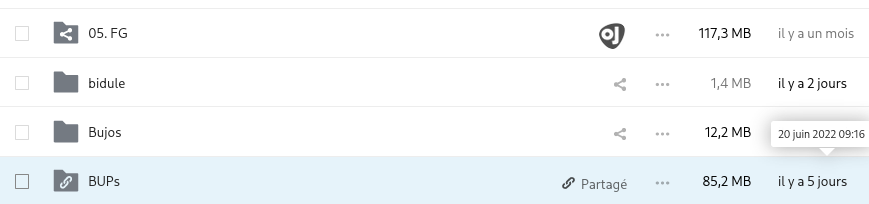
\includegraphics{./Captures/nuage.partager.icones.png}
	\caption{Deux exemples de ressources partagées et deux autres non partagées.}
\end{figure}
Ainsi, le dossier \og~O5 FG~\fg{} a été utilisé par un autre utilisateur dont les initiales sont OJ (puisqu'aucun avatar ne semble avoir été défini par l'utilisateur). 
Le dossier \og~BUPs~\fg{} par contre fait l'objet d'un partage de ma part. 
Il est intéressant de noter que les icônes représentant ces deux ressources et les deux autres (Bidule et Bujos) diffèrent et que suivant le sens du partage le motif superposé à l'icône n'est pas le même. 

\subsection{Les options de partage avancées}
%\addcontentsline{toc}{subsection}{Les options du partage}
Pour avoir  plus de détails il suffit soit de cliquer sur l'icône \ldots soit sur l'icône de partage et alors le volet latéral des propriétés de partage apparaîtra.
\begin{figure}
	\centering
	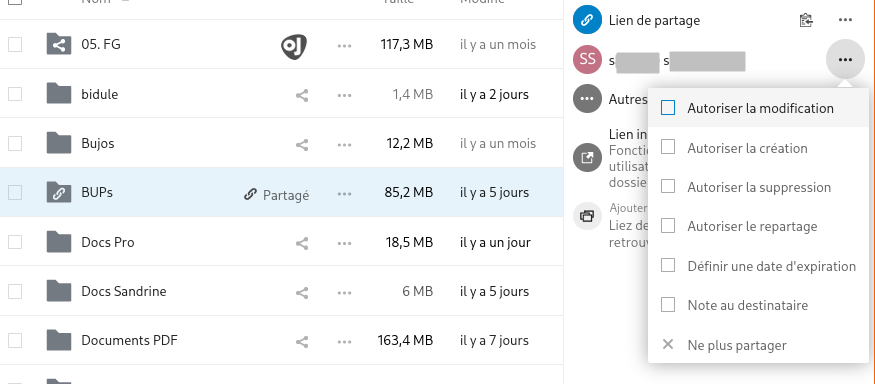
\includegraphics{./Captures/nuage.partager.menu.contextuel.png}
	\caption{Les différentes possibilités de partage offertes.}
\end{figure}

On voit par la dernière capture qu'il est possible de gérer les droits de modification, de création ou de suppression sur la ressource, mais aussi d'autoriser le repartage et, plus intéressant encore, de définir un mot de passe d'accès et une date d'expiration du partage.

\section{Créer un lien vers une ressource extérieure.}
Il peut être pratique de conserver sous forme de fichier un lien vers une ressource internet. 
Dans mon établissement ce type de fichier m'est très pratique pour déployer sur tous les postes accueillant les évaluations des élèves de 6\ieme{} en utilisant un fichier sur un espace de stockage partagé en interne dans l'établissement et en le copiant de poste en poste --nous n'avons pas de domaine, ni de politique de déploiement par GPO-- du coup le fichier \texttt{.url} contient le lien qui sera ouvert par le navigateur par défaut de la machine vers le site web de passation des épreuves. 

%\newpage % force le passage sur une nouvelle page pour que les colonnes restent bien comme il faut, au besoin
\begin{multicols}{2}
Tout commence par le menu $\oplus$ \ldots
\begin{figure}
	\centering
	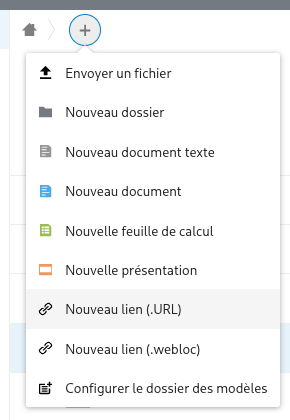
\includegraphics{./Captures/nuage.menu.plus.zoom.png}
	\caption{Le menu $\oplus$.}
\end{figure}
\columnbreak

Je sélection la ligne pour les URL.
\begin{figure}
	\centering
	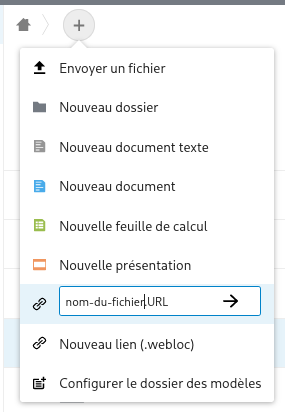
\includegraphics{./Captures/nuage.menu.plus.creer.url.png}
	\caption{Nommage du raccourcis}
\end{figure}
\end{multicols}

Je choisis de nommer par \texttt{nom-du-fichier} le fichier \texttt{.URL} qui sera généré, il contiendra un lien vers le site \url{https://ctan.org}~:
\begin{figure}
	\centering
	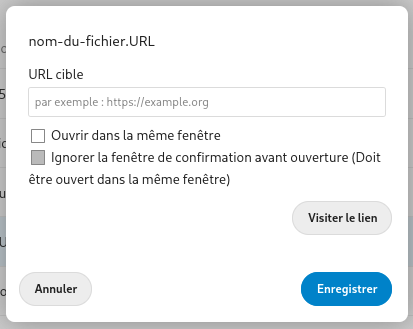
\includegraphics[width=0.333\linewidth]{./Captures/nuage.url.proprietes.png}
	\caption{Les propriétés du lien.}
\end{figure}

et je règle les options relatives à son ouverture (même fenêtre, fenêtre de confirmation, \ldots), ce qui fait qu'en cliquant sur le lien, la mini fenêtre suivante va s'afficher :
\begin{figure}
	\centering
	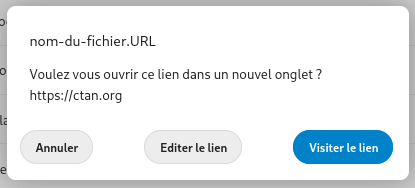
\includegraphics[width=0.333\linewidth]{./Captures/nuage.url.fenetre.confirmation.png}
	\caption{Confirmation de l'ouverture du lien.}
\end{figure}

Le site s'ouvre alors dans un nouvel onglet conformément aux propriétés réglées antérieurement.
\begin{figure}
	\centering
	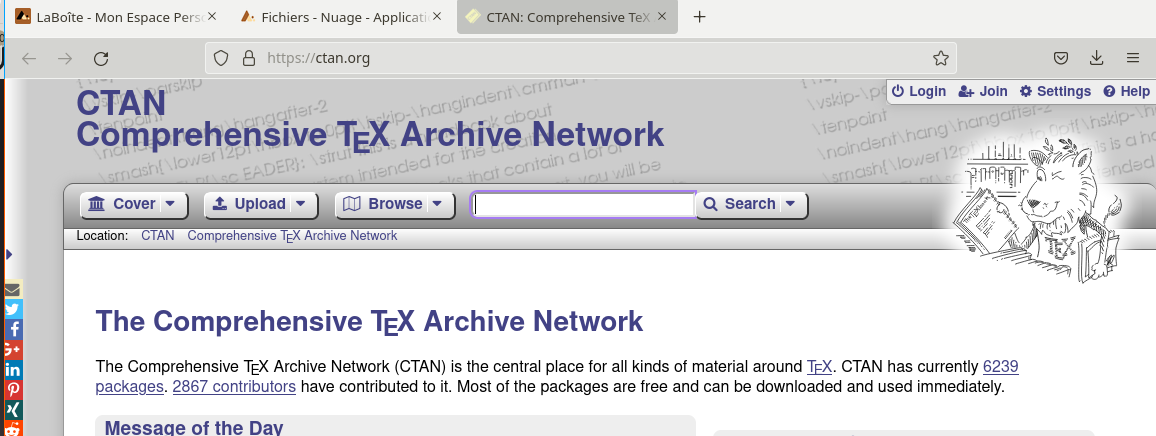
\includegraphics{./Captures/nuage.url.ouverture.nouvel.onglet.png}
	\caption{Le site CTAN.org est désormais ouvert dans un nouvel onglet.}
\end{figure}

\section{Libreoffice \emph{online}}

Au sein du nuage, \emph{LibreOffice OnLine\/} ou encore LOOL a été intégrée, toujours dans le menu $\oplus$ et offre le traitement de textes \emph{writer\/}, le tableur \emph{calc\/} et le logiciel de présentation \emph{impress\/}, permettant d'ouvrir les document montés sur le nuage mais aussi d'éditer ceux déjà présents.

Ainsi vous accéderez aux trois outils de la suite bureautique libreoffice online les plus utilisés, le traitement de textes \emph{writer\/}, le tableur \emph{calc\/} et le logiciel de présentations \emph{impress\/} comme le montrent les captures suivantes.

\begin{figure}
    \centering
    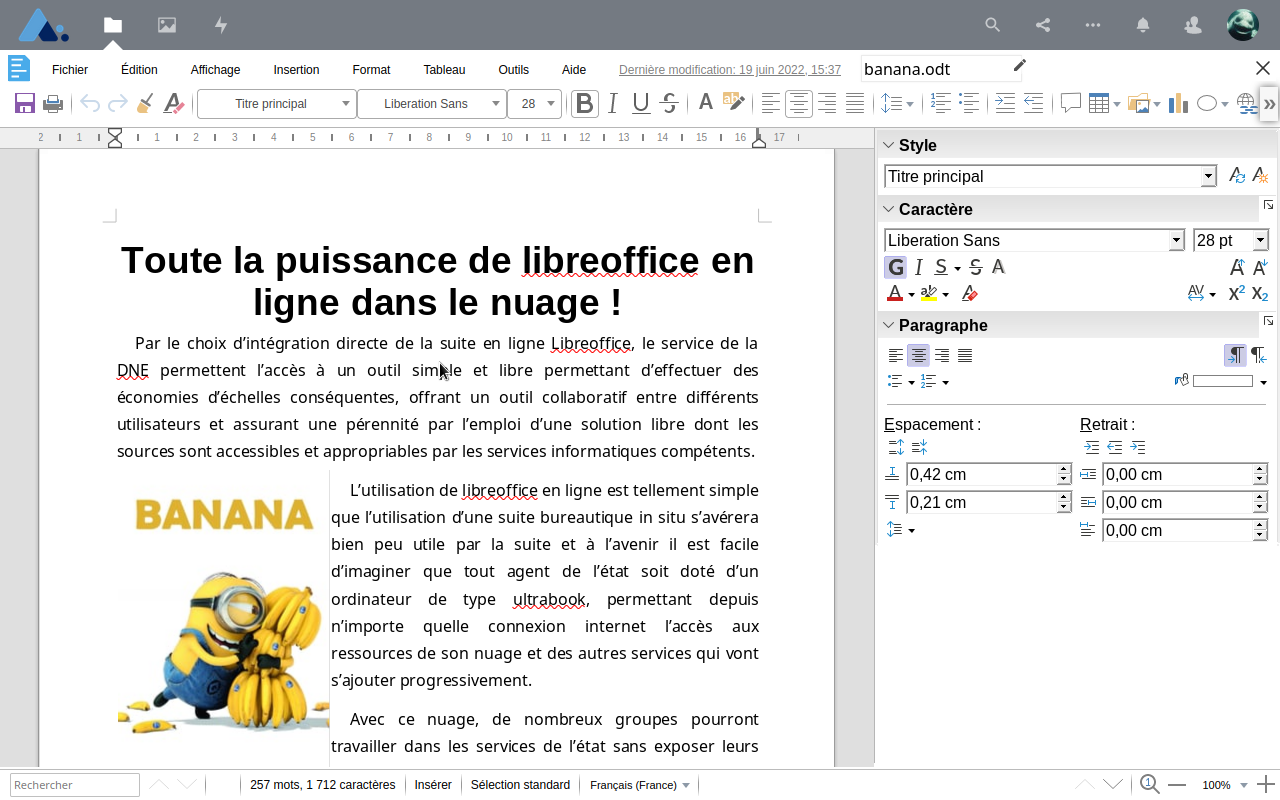
\includegraphics[]{Captures/nuage.lool.writer.png}
    \caption{Exemple de fichier de traitement de textes composé dans Libreoffice \emph{writer\/} au sein du nuage.}
\end{figure}

La capture d'écran ci-avant montre un document rédigé entièrement en ligne, inclusion d'image comprise, avec le volet latéral de Libreoffice actif.

Il faut prendre en compte quelques points néanmoins, l'un d'entre eux est qu'à l'instar de la suite \emph{Office\/} de Microsoft\textregistered{} la version en ligne n'est pas complète mais une version allégée. 
Les utilisateurs avancés de Libreoffice se verront amputés de quelques fonctionnalités, par exemple en ce qui me concerne, l'éditeur d'équations.
Notez cependant qu'un fichier édité en local, \emph{i.e.\/} sur un ordinateur directement par la version complète de Libreoffice sera conservé lors du transfert, et, s'il y a ouverture, sera considéré comme un objet inséré dans le document malgré l'impossibilité d'éditer directement son contenu.

\begin{figure}
    \centering
    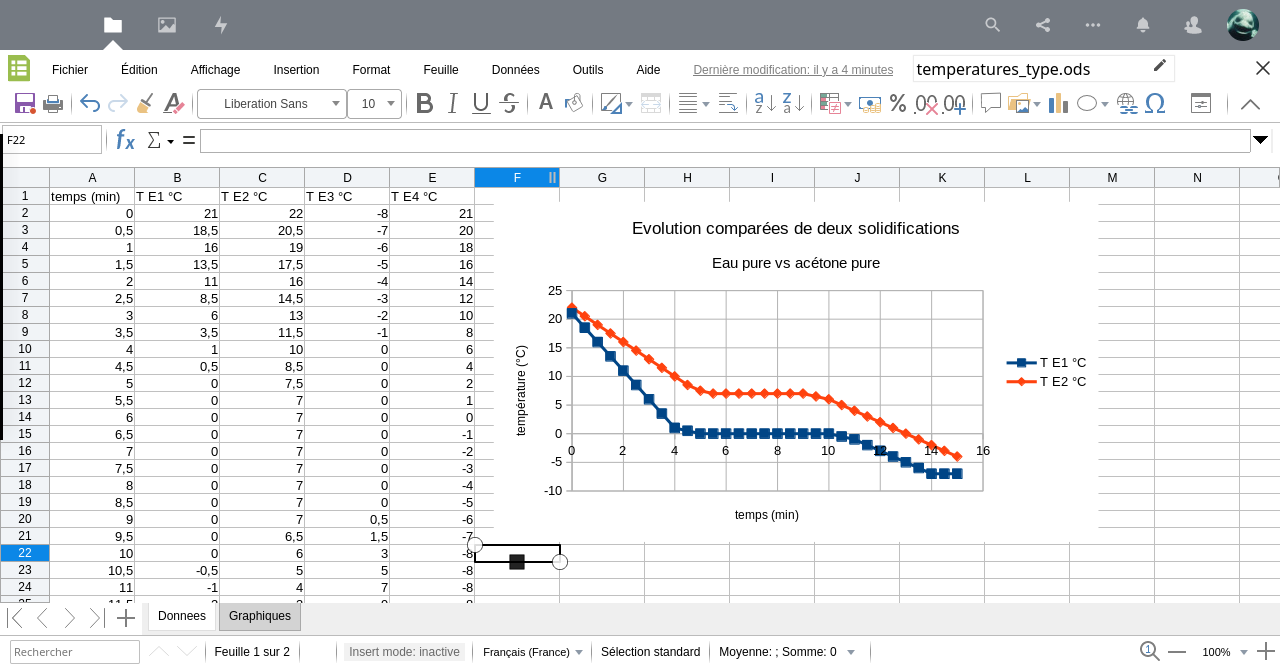
\includegraphics[]{Captures/nuage.lool.tableur.png}
    \caption{Un exemple de tableur/grapheur sous Libreoffice \emph{Calc\/} et un graphique inséré, le tout directement en ligne.}
\end{figure}

Le tableur permet l'édition de formules et l'insertion de graphiques, comme on pouvait l'espérer.

\begin{figure}
    \centering
    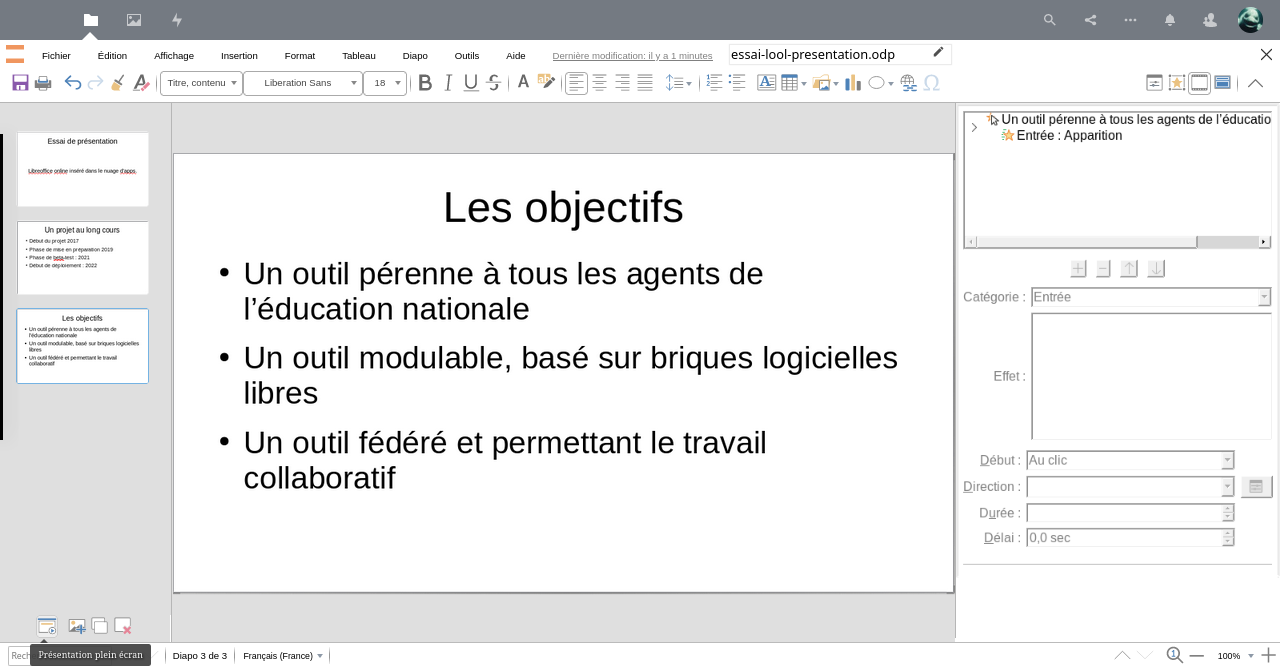
\includegraphics[]{Captures/nuage.lool.presentation.png}
    \caption{Une ébauche de présentation de Libreoffice \emph{Impress\/} en plein développement.}
\end{figure}

Et évidemment il est possible de créer des présentations simples voire complexes le tout en ligne, ou de les modifier.

La suite bureautique Libreoffice Online permet aussi d'exporter, et \emph{de facto} de télécharger les documents produits dans divers formats, l'exemple suivant montre les exportations associées à \emph{Writer\/}.

\begin{figure}
    \centering
    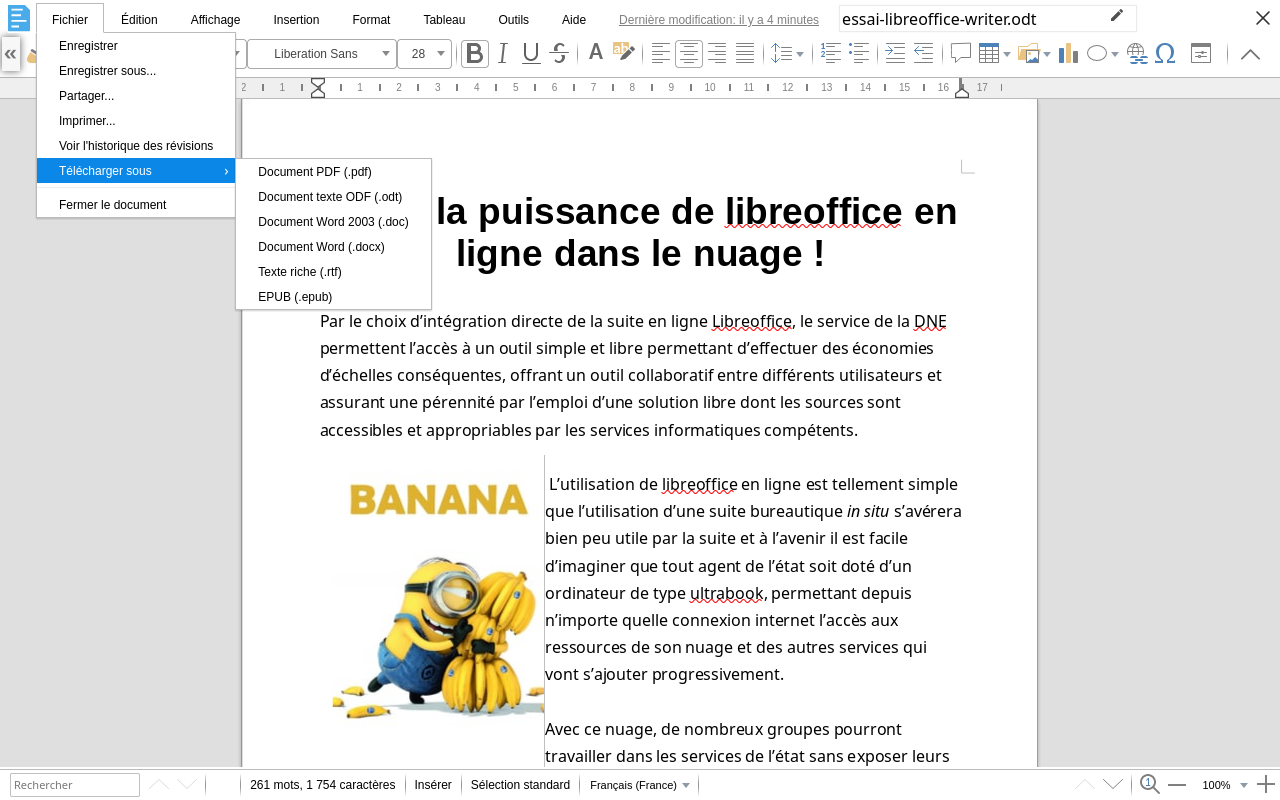
\includegraphics[]{Captures/nuage.lool.writer.exportations.png}
    \caption{Les exportations proposées dans Libreoffice \emph{writer\/}.}
\end{figure}

Cette fois-ci vous aurez noté que le volet latéral est occulté.